% !TEX encoding   = UTF8
% !TEX spellcheck = ru_RU
% !TEX root = seminars.tex

%%==================
\chapter{Приложение}
%%==================
%%===========================================
\section{Установка и настройка рабочей среды}\label{sect:workEnv}
%%===========================================
{ % hot keys
\newcommand*{\hotkey}[1]{\fbox{\texttt{\small #1}}}
\newcommand*{\hotplus}{{\small\,+\,}}
\newcommand*{\hotkeys}[2]{\hotkey{#1}\hotplus\hotkey{#2}}
\newcommand*{\hotkeyss}[3]{\hotkey{#1}\hotplus\hotkey{#2}\hotplus\hotkey{#3}}



%%============================
\paragraph{ОС \name{Windows}.}
%%============================
Мы настоятельно рекомендуем в качестве \name{IDE} установить \name{Qt\,Creator}. Совместно с ним используйте \name{MinGW-w64} (компилятор, компоновщик, отладчик и прочее).

Удобная \name{UNIX}-подобная командная среда \name{Git\,Bash} идёт в комплекте с системой контроля версий \href{\giturl}{\git}, которая, в свою очередь, входит в состав \name{Smartgit}-а "--- графической облочки над \git-ом. Командная среда, помимо прочего, облегчит тестирование программ в автоматическом и полуавтоматическом режимах. А система контроля версий окажется неотъемлемым элементом разработки сложных программ.

Для установки и настройки компонентов:
\begin{itemfeature}
\item Загрузите \href{\qtcreatorurl}{\name{Qt\,Creator}}\footnote{\nolinkurl{\qtcreatorurl}}, \href{\mingwurl}{\name{MinGW-w64}}\footnote{\nolinkurl{\mingwurl}} и \href{\smartgiturl}{\name{Smartgit}}\footnote{\nolinkurl{\smartgiturl}}.

\item Распакуйте архив \name{MinGW-w64} в каталог \code{c:\backslash{}Program Files} или любой другой каталог, куда вы обычно устанавливаете программы.

И далее, следуя графическим инструкциям из архива
\begin{flushleft}
	\yadisk{cpp-seminars/how-to-s/how-to\_set-up-qt-creator.zip},
\end{flushleft}
выполните последующие пункты.

\item Добавьте путь к компилятору в список стандартных системных путей. Если вы не знаете, как это выполнить

\item Установите \name{Qt\,Creator}, следуя инструкциям установщика.

\item Запустите \name{Qt\,Creator}. Откройте окно настройки параметров из меню \code{Инструменты} \code{->} \code{Параметры}. Во вкладке \code{Комплекты} выберите, скорее всего, единственный комплект \code{Desktop}. В качестве компиляторов для \lang{C} и \lang{C++} выберите из списка \code{MinGW} \GCC{} \code{C} и \code{C++}, соответственно. В качестве отладчика укажите \GDB.

\item Установите \name{Smartgit}, оставляя рекомендуемые (по умолчанию) параметры в тех местах, где вы сомневаетесь, что выбрать.
\end{itemfeature}

Если что-то пошло не так, повторите процедуру \textbf{спокойно}, выполняя \textbf{в точности} все указанные выше действия. Используйте только латиницу для каталогов установки и проектов, иногда русские буквы в путях приводят к ошибкам в \name{Qt\,Creator}-е.

И теперь не получилось? Хм-м... Тогда обратитесь за помощью к студентам старших курсов или преподавателю.



%%=========================
\paragraph{ОС \name{UNIX}.}
%%=========================
Пользователи \name{UNIX} и подобных ей операционных систем могут установить при помощи системы управления пакетами (например, \code{apt} в \name{Ubuntu}) дистрибутив \name{Qt\,Creator} совместно со средствами сборки \name{GNU} \GCC{} или \code{Clang}, а также систему контроля версий \git{} и \name{Smartgit}.



%%=============================
\section{Редактирование текста}\label{sect:typing}
%%=============================
Набор исходного текста "--- неотъемлемая часть разработки программ. Используйте <<горячие>> клавиши для более быстрого редактирования. Краткий список наиболее популярных комбинаций, поддерживаемых даже простыми редакторами:

\begin{longtable}[l]{@{}rp{0.7\textwidth}@{}}
\endhead
\endfoot

\hotkeys{Ctrl}{A}  & Выделить всё.\\[0.5em]

\hotkeys{Ctrl}{C}  & Скопировать выделение. \\
\hotkeys{Ctrl}{V}  & Вставить. \\[0.5em]

\hotkeys{Ctrl}{Z}  & Отменить последнее действие. \\[0.5em]

\hotkey{Home} & Переместить курсор в начало\slash{}конец текущей строки. \\
\hotkey{End}  & \\[0.5em]

\hotkeys{Shift}{Home} & Выделить символы с текущей позиции и до начала\slash{}конца строки. \\
\hotkeys{Shift}{End}  & \\[0.5em]

\hotkeys{Ctrl}{Home} & Переместить курсор в начало\slash{}конец файла. \\
\hotkeys{Ctrl}{End}  & \\[0.5em]

\hotkeys{Ctrl}{\leftarrow}  & Переместить курсор по словам. \\
\hotkeys{Ctrl}{\rightarrow} & \\
\end{longtable}

\noindent Дополнительные полезные комбинации в \name{Qt\,Creator}:
\begin{longtable}[l]{@{}rp{0.7\textwidth}@{}}
\endhead
\endfoot

\hotkeys{Ctrl}{I} & Выровнять отступ (\textenglish{\textbf{i}ndent}) текущей строки или выделения. \\[0.5em]

\hotkeys{Ctrl}{\slash} & Комментировать\slash{}раскомментировать текущую строку или выделение. \\[0.5em]

\hotkeyss{Ctrl}{Shift}{R} & Переименовать имя под курсором. \\[0.5em]

\hotkeyss{Ctrl}{Shift}{\uparrow}   & Сместить текущую строку вверх\slash{}вниз. \\
\hotkeyss{Ctrl}{Shift}{\downarrow} & \\[0.5em]

\hotkeyss{Alt}{Shift}{\uparrow}   & Редактировать столбец. \\
\hotkeyss{Alt}{Shift}{\downarrow} & \\
\end{longtable}

Полезно научиться набирать текст вслепую, то есть не глядя на клавиатуру. В сочетании с использованием горячих клавиш это позволяет достичь существенного ускорения при работе с исходным кодом. Таким образом, остаётся больше времени для размышлений над структурой и логикой самой программы. В качестве примера он-лайн клавиатурного тренажёра приведём \href{\typingtutorurl}{эту}\footnote{\nolinkurl{\typingtutorurl}} ссылку.

} % hot keys



%%====================
\section{Unix утилиты}\label{sect:utils}
%%====================
Совместно с командной средой (\name{bash} "--- \textenglish{\textbf{b}ourne \textbf{a}gain \textbf{sh}ell}) поставляется широкий набор полезных программ, или утилит (\textenglish{utilities}).

\console/$ cd dir/%$

\textenglish{\textbf{c}hange \textbf{d}irectory} "--- перейти в каталог \code{dir}. Если каталог опущен, то перейти в домашний каталог. (Определяется значением переменной среды \code{HOME}.) Файловая система \textenglish{Unix} представляет собой единое дерево, и любой абсолютный путь начинается с корня (\code{/}). Точка (\code{.}) означает текущий каталог, две точки (\code{..}) "--- родительский каталог.

\console/$ cd ../%$

Перейти в родительский каталог.

\console|$ cd /|%$

Перейти в корневой каталог.

\console/$ pwd/%$

\textenglish{\textbf{p}rint \textbf{w}orking \textbf{d}irectory} "--- вывести на экран абсолютный путь к текущему каталогу.

\console/$ ls dir/%$

\textenglish{\textbf{l}i\textbf{s}t} "--- вывести на экран содержимое каталога \code{dir}. Если каталог опущен, то по умолчанию используется текущий каталог.

\console/$ man cmd/%$

\textenglish{\textbf{man}ual} "--- вывести на экран подробную справку о команде \code{cmd}.

\console/$ cmd --help/%$

Вывести на экран короткую справку о команде \code{cmd}. Полезно, если утилита \code{man} недоступна.

\console/$ mkdir dir/%$

\textenglish{\textbf{m}a\textbf{k}e \textbf{dir}ectory} "--- создать каталог \code{dir}.

\console/$ rmdir dir/%$

\textenglish{\textbf{r}e\textbf{m}ove \textbf{dir}ectory} "--- удалить пустой каталог \code{dir}.

\console/$ rm file/%$

\textenglish{\textbf{r}e\textbf{m}ove} "--- удалить файл. Используя опцию \code{-r} можно рекурсивно удалить непустой каталог.

\console/$ mv src dst/%$

\textenglish{\textbf{m}o\textbf{v}e} "--- перемещает/переименовывает файл \code{src} в \code{dst}. Имя \code{dst} может быть каталогом, тогда \code{mv} перемещает \code{src} туда.

\console/$ cat file.../%$

\textenglish{\textbf{cat}enate} "--- связывает файлы и выводит объединённое содержимое на экран.

\console/$ less file/%$

Более мощный аналог утилиты \code{more} "--- постраничного фильтра для просмотра файлов. Часто применяется для буферизации вывода на экран, используя конвейер:

\console/$ odjdump -d prog | less/%$


\console/$ vim file/%$

\textenglish{\textbf{v}isual editor \textbf{im}proved} "--- открыть файл для редактирования. Пройти вводный курс по использованию этого мощного редактора можно запустив команду:

\console/$ vimtutor/%$



%%==================================
\section{Интерпретатор \name{shell}}\label{sect:shell}
%%==================================
Когда система (в терминале) выдаёт приглашение \code{\$} и вы вводите команды для выполнения, вы имеете дело не с ядром самой системы, а с неким посредником, называемым интерпретатором команд, или \name{shell}\footnote{Более подробно об интерпретаторе \name{shell} и других возможностях системы \textenglish{Unix} излагается, например, в книге \fullcite{Kernighan:1992:ru}}. Это обычная программа, но она может делать удивительные вещи. Применение программы--посредника обеспечивает три главных преимущества:

\begin{itemfeature}[itemsep=\baselineskip]
  \item Сокращённые имена файлов: можно задать целое множество файлов в качестве аргументов команде, указав шаблон для имён: \name{shell} будет искать файлы, имена которых соответствуют заданному шаблону.

  \console/$ ls *.cpp *.c/%$

  Вывести на печать имена всех файлов в текущем каталоге, которые оканчиваются на~\code{.cpp} или \code{.c}. Символ \code{*} в шаблоне соответствует любой последовательности символов. Поддерживаются и другие специальные символы для задания шаблона.


  \item Переключение ввода--вывода: вывод любой программы можно направить в файл, а не на терминал, ввод можно получать из файла, а не с терминала. Ввод и вывод можно даже передать другим программам.

  \console/$ ls *.cpp > cppfiles.txt/%$

  Имена всех файлов, оканчивающихся на~\code{.cpp}, направить в файл \code{cppfiles.txt}. Файл будет создан, если не существует, или перезаписан, если существует.

  \console/$ wc -l < main.cpp/%$

  Подсчитать количество строк (опция \code{-l}) в файле \code{main.cpp}.

  \console/$ cat main.cpp | wc -l/%$

  То же. Символ~\code{|} обозначает конвейер. Вывод команды слева передаётся на ввод команде справа. Можно организовывать в конвейере цепочку любой длины.

  \console/$ wc -l main.cpp/%$

  То же, используя лишь возможности самой утилиты \code{wc} (\textenglish{\textbf{w}ord \textbf{c}ount}).


  \item Создание собственной среды: можно определить свои собственные команды и правила сокращений.
\end{itemfeature}



%%==========================================
\section{Рисование графиков в \lang{Python}}\label{sect:pyplot}
%%==========================================
Каждый язык имеет свои достоинства и недостатки и, как правило, нацелен на эффективное решение определённого класса задач. Совместное использование разных языков часто помогает сократить усилия при разработке программ и повысить гибкость либо удобство создаваемых инструментов. Попробуем продемонстрировать это на примере визуализации результатов обработки данных лабораторной работы по физике, которые можно получить методом наименьших квадратов, рассмотренным в разделе~\ref{chap:helloworld} (также см. упр.~\ref{ex:plot} на странице~\pageref{ex:plot}).

\begin{figure}[ht]
  {\centering
    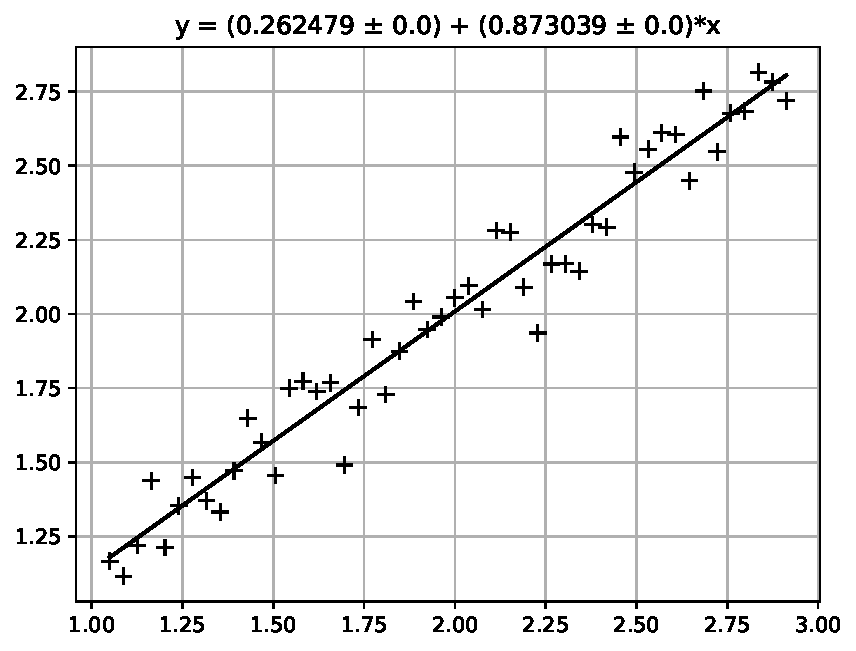
\includegraphics[width=0.6\textwidth]{images/line_approx.pdf}

  }
  \caption{Визуализация при помощи \name{Matplotlib}}
  \label{fig:pyplot}
\end{figure}

В языке \lang{C++} нет встроенных графических средств. Для этого необходимо использовать сторонние библиотеки. Работа с подобными инструментами не всегда настолько проста, как хотелось бы. А настройка внешнего вида координатных осей, изображаемых кривых и точек может потребовать перекомпиляции всей программы.

Одним из действительно удобных для этого случая решений является написание сценария (\textenglish{script}) на интерпретируемом языке. \href{\pythonurl}{\lang{Python}} относится к этому ряду языков и имеет мощную поддержку разнообразных средств практически прямо <<из коробки>>. Ниже приведён вариант решения нашей задачи с использованием пакета \href{\matplotliburl}{\name{Matplotlib}}.

\begin{center}
  \yadisk{cpp-seminars/examples/01/plot.py}
\end{center}

\inputminted[linenos, fontsize=\small]{py}{01/src/plot.py}

Совместить использование разработанных нами отдельных инструментов можно при помощи командной среды. Для этого достаточно всего одной строки (см. страницу~\pageref{sect:shell}):
\begin{consolecode}
$ ./lsm line_approx.txt | xargs python3 plot.py
\end{consolecode}

\noindent Результат в виде графического файла \code{line\_approx.pdf}, изображён на рисунке~\ref{fig:pyplot}.
